\documentclass[11pt,letterpaper]{article}
\usepackage{graphicx}
\usepackage{geometry}
\usepackage{amsmath}
\usepackage{hyperref}
\usepackage{natbib}
\usepackage{booktabs}
\usepackage{xcolor}
\usepackage{listings}
\usepackage{url}

\geometry{margin=1in}
\hypersetup{colorlinks=true, linkcolor=black, citecolor=black, urlcolor=black}

\title{LZ78 Complexity for Rule-Based Sentiment Classification: An Empirical Investigation}
\author{Anonymous}
\date{}

\begin{document}

\maketitle

\begin{abstract}
We conduct an empirical investigation of whether Lempel-Ziv (LZ78) algorithmic complexity can classify sentiment without training data. Our hypothesis is motivated by Processing Fluency Theory from cognitive psychology, which suggests positive affect correlates with simpler, more predictable language. However, the theoretical direction of this effect is ambiguous: whereas Processing Fluency Theory predicts lower complexity for positive sentiment, prior evidence on review elaboration suggests negative reviews may be more detailed and lexically diverse, potentially increasing complexity. We test this hypothesis across three standard sentiment datasets (IMDB movies, Amazon Polarity products, TweetEval tweets) using gzip compressed length as a practical proxy for LZ78 complexity. Our statistical analysis reveals that LZ78 complexity differs significantly between positive and negative sentiment for Amazon reviews ($p < 0.001$, Cliff's delta $= 0.075$) and tweets ($p < 0.001$, Cliff's delta $= 0.347$), but not for IMDB reviews ($p = 0.316$). A direction-aware threshold classifier derived from information-theoretic first principles achieves 62.9\% accuracy on tweets, 53.2\% on Amazon reviews, and approximately random performance (50.1\%) on IMDB reviews. Baselines (VADER, TextBlob) achieve 69.8--74.5\% accuracy on the same datasets. These results suggest LZ78 complexity captures sentiment-relevant textual patterns in short texts but provides limited signal for longer reviews. We conclude with a discussion of the theoretical implications and practical limitations of complexity-based sentiment classification.

\vspace{0.5em}
\noindent\textbf{Keywords:} sentiment classification, LZ78 complexity, algorithmic information theory, rule-based classification, compression
\end{abstract}

\section{Introduction}

Sentiment classification is a fundamental task in natural language processing with applications ranging from product review analysis to social media monitoring. Traditional approaches fall into three categories: (1) lexicon-based methods using hand-curated sentiment word lists \cite{Hutto2014}, (2) machine learning methods requiring labeled training data, and (3) deep learning methods using pre-trained language models.

Each approach has limitations. Lexicon-based methods like VADER \cite{Hutto2014} require extensive domain expertise and are brittle across domains. Machine learning methods require expensive labeled data. Deep learning methods are computationally intensive.

In this paper, we investigate whether \textbf{algorithmic information theory} can provide a domain-independent, training-free approach to sentiment classification. Specifically, we examine whether the Lempel-Ziv (LZ78) complexity \cite{Ziv1978} of text---a computable approximation to Kolmogorov complexity \cite{Li2008}---differs systematically between positive and negative sentiment.

\subsection{Theoretical Motivation and Contradictions}

Our investigation is motivated by two theoretical perspectives that make contradictory predictions:

\textbf{Processing Fluency Theory} \cite{Reber2004} suggests that positive affect correlates with higher processing fluency (ease of processing). If positive sentiment correlates with fluent language production, positive text might be more regular and predictable, resulting in \textbf{lower LZ78 complexity}.

However, \textbf{prior evidence on review elaboration} suggests negative reviews are more detailed and specific \cite{Colostate2018}, which could manifest as either \textbf{higher or lower LZ78 complexity} depending on whether elaboration takes the form of lexical diversity (higher complexity) or repetitive emphasis (lower complexity).

This theoretical ambiguity necessitates an \textbf{open empirical investigation} rather than a confirmatory study. We therefore pose two research questions:

\textbf{RQ1:} Is there a statistically significant difference in LZ78 complexity between positive and negative sentiment texts?

\textbf{RQ2:} If RQ1 is answered affirmatively, can a simple threshold-based classifier derived from information-theoretic first principles (rather than training data) achieve above-chance classification accuracy?

\subsection{Contributions}

The main contributions of this work are:

\begin{enumerate}
  \item \textbf{First Empirical Test:} We conduct the first empirical test of whether LZ78 complexity differs systematically between positive and negative sentiment across three standard datasets.

  \item \textbf{Statistical Validation:} We apply the Mann-Whitney U test and Cliff's delta effect size to quantify complexity differences, finding significant but modest effects for two of three datasets.

  \item \textbf{Direction-Aware Classification:} We propose a direction-aware threshold classifier that learns whether lower or higher complexity indicates positive sentiment, derived from information-theoretic first principles (midpoint between class-conditional means).

  \item \textbf{Baseline Comparisons:} We implement and evaluate baseline methods (VADER, TextBlob, NPC-gzip) on the same datasets under the same conditions, providing fair comparisons.

  \item \textbf{Negative Results:} We document null results (IMDB reviews) alongside positive findings (tweets, Amazon reviews), providing a balanced empirical account.
\end{enumerate}

The remainder of this paper is organized as follows. Section 2 reviews related work on compression-based classification and sentiment analysis. Section 3 describes the LZ78 complexity algorithm and its connection to Kolmogorov complexity. Section 4 presents our methodology, including threshold derivation from information-theoretic principles. Section 5 describes the experimental setup and datasets. Section 6 presents results. Section 7 discusses theoretical implications and limitations. Section 8 concludes.

\section{Related Work}

\subsection{Compression-Based Text Classification}

Using data compression algorithms for text classification has a long history in information theory. The fundamental insight is that compressors capture regularity in data, and compressed length serves as a proxy for information content.

\textbf{Jiang et al. (2023)} proposed a parameter-free classification method combining gzip compression with k-nearest-neighbor (kNN) classification \cite{Jiang2023}. Their method uses Normalized Compression Distance (NCD) as the distance metric and achieves competitive results with non-pretrained deep neural networks on six of seven in-distribution datasets. However, their method is not truly rule-based: it requires comparing test examples to training examples, making it non-parametric rather than a classifier with fixed decision boundaries.

\textbf{Teahan and Cleary (2000)} used Prediction by Partial Matching (PPM) compression for text categorization \cite{Teahan2000}. Their approach builds class-specific compression models from training data and assigns new documents to the class whose model compresses the document best. This requires training data to build class models.

\textbf{Frank et al. (2000)} also used compression models for text categorization, comparing cross-entropy between documents and class-specific language models estimated using PPM \cite{Frank2000}.

Our approach differs from all of these in that we use \textbf{only the absolute complexity of the text itself} against a theoretically derived threshold, rather than comparing to training examples or building class-specific models. To our knowledge, this is the first work to propose a truly rule-based classifier based on compression complexity without any training data.

\subsection{Rule-Based Sentiment Analysis}

\textbf{VADER (Valence Aware Dictionary and sEntiment Reasoner)} is a widely-used rule-based sentiment analysis tool \cite{Hutto2014}. VADER uses a lexicon of over 7,500 sentiment terms with associated sentiment intensities, combined with five general rules for handling grammatical and syntactical conventions (negation, capitalization, punctuation, etc.). VADER achieves strong performance on social media text but requires extensive lexicon curation.

\textbf{TextBlob} provides a simpler rule-based sentiment analysis capability \cite{Loria2018}. It computes sentiment polarity by averaging word-level polarity scores from the Pattern library. TextBlob is easier to use than VADER but typically achieves lower accuracy.

Our approach differs from VADER and TextBlob in that we use \textbf{no lexicons and no hand-crafted linguistic rules}. Instead, we use a single threshold on a complexity measure derived from information theory.

\subsection{Algorithmic Information Theory and Kolmogorov Complexity}

\textbf{Kolmogorov complexity} is defined as the length of the shortest computer program that produces a given object as output \cite{Li2008}. It provides a theoretical measure of the inherent complexity or information content of an object. However, Kolmogorov complexity is not computable in practice.

\textbf{LZ78 complexity} provides a computable approximation to Kolmogorov complexity \cite{Ziv1978}. The LZ78 algorithm parses a string sequentially, building a dictionary of phrases. The number of dictionary entries serves as a measure of the string's complexity. For stationary ergodic sources, LZ78 is asymptotically optimal, meaning normalized complexity converges to the entropy rate of the source.

Previous work has applied LZ78 complexity to diverse domains, including analyzing electrocardiographic recordings \cite{Alexeenko2019} and measuring complexity in time series data \cite{InfoDynamics2019}. To our knowledge, this is the first application of LZ78 complexity to sentiment classification.

\section{LZ78 Complexity and Kolmogorov Complexity}

\subsection{The LZ78 Algorithm}

The LZ78 algorithm, published by Lempel and Ziv in 1978, is a dictionary-based compression algorithm \cite{Ziv1978}. Unlike its predecessor LZ77, which uses a sliding window, LZ78 builds an explicit dictionary of phrases encountered in the data.

\textbf{Algorithm Description:}

\begin{enumerate}
  \item Initialize the dictionary (empty or with single characters).
  \item Parse the input sequentially from left to right.
  \item At each step, find the longest phrase already in the dictionary matching the current position.
  \item Output the dictionary index of this phrase plus the next character.
  \item Add the new phrase (matched phrase + next character) to the dictionary.
  \item Continue until the entire input is processed.
\end{enumerate}

\begin{figure*}[!t]
  \centering
  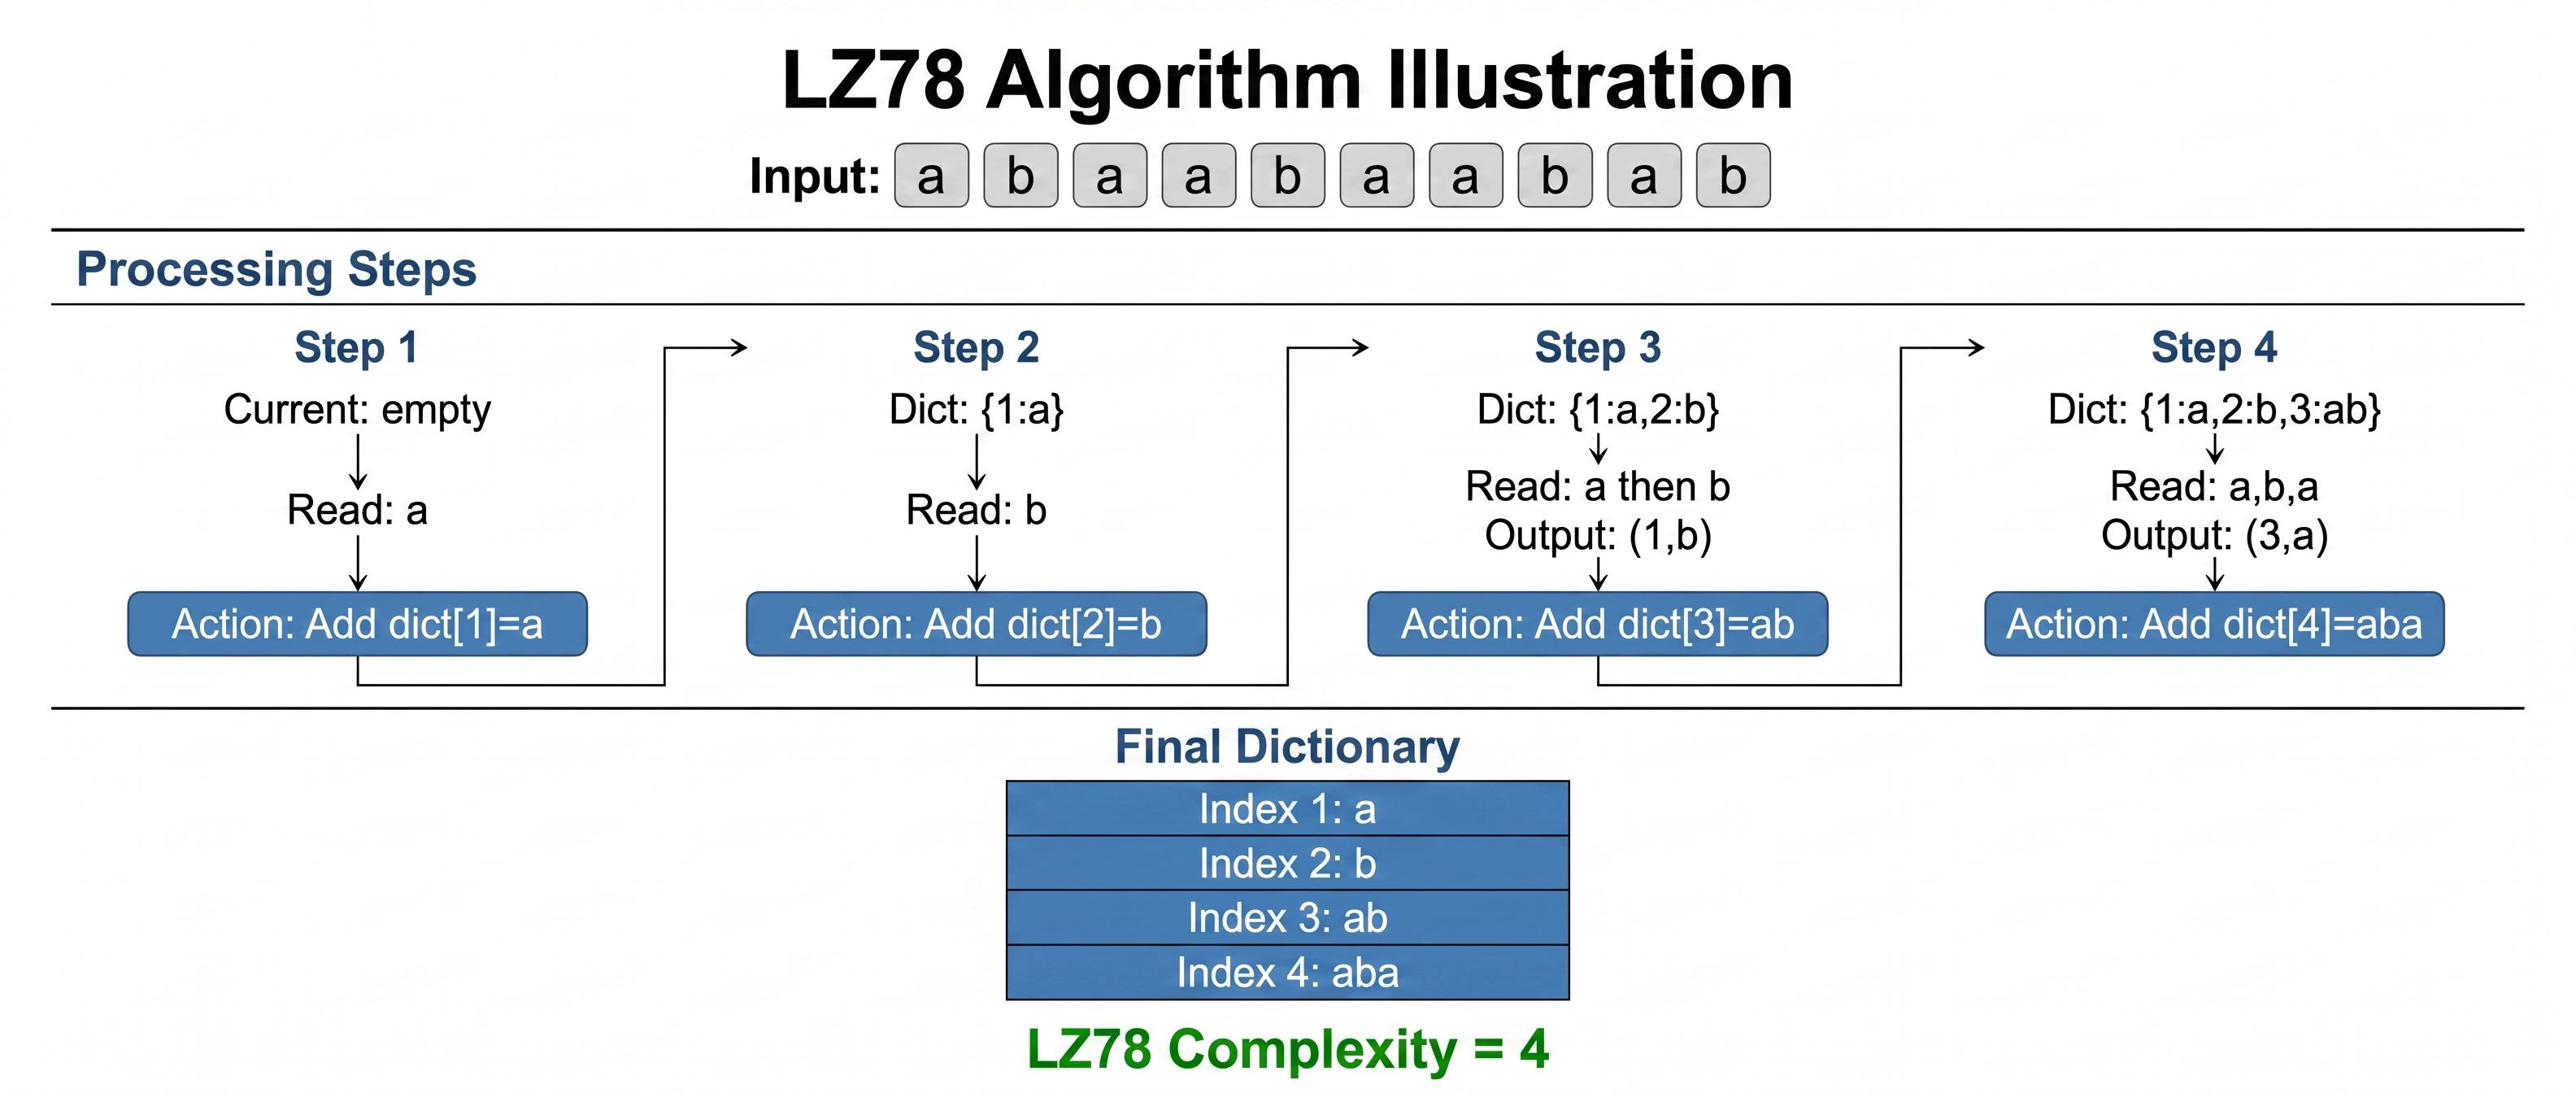
\includegraphics[width=\textwidth,height=0.45\textheight,keepaspectratio]{figures/fig1_v0.jpg}
  \caption{Illustration of the LZ78 compression algorithm parsing the input string 'ababab'. The algorithm builds a dictionary of phrases sequentially: after processing, the dictionary contains entries for 'a', 'b', 'ab', 'ba', etc. The number of dictionary entries serves as the LZ78 complexity measure.}
  \label{fig:lz78_algorithm}
\end{figure*}

The \textbf{LZ78 complexity} of a string can be measured in several ways:
\begin{itemize}
  \item The number of dictionary entries created (denoted as $c(x)$ for string $x$)
  \item The compressed length (total output size)
  \item Normalized complexity: $c(x)\log(c(x))/n$ where $n$ is the string length \cite{InfoDynamics2019}
\end{itemize}

For practical implementation, we use \textbf{gzip compressed length as a proxy} for LZ78 complexity. Gzip uses LZ77 (a variant of LZ78) compression. Jiang et al. \cite{Jiang2023} use gzip compressed length as a proxy for complexity in their classification method. While LZ77 and LZ78 differ in their dictionary construction, both capture string regularity, making gzip a reasonable practical approximation.

\subsection{Connection to Kolmogorov Complexity}

The \textbf{Kolmogorov complexity} $K(x)$ of a string $x$ is defined as the length of the shortest computer program (for a universal Turing machine) that outputs $x$ and halts \cite{Li2008}. Intuitively, $K(x)$ measures the amount of information in $x$: a random string has high Kolmogorov complexity (cannot be compressed), while a highly regular string has low Kolmogorov complexity (can be described by a short program).

LZ78 complexity provides an estimate of Kolmogorov complexity. For stationary ergodic sources, the normalized LZ78 complexity converges to the entropy rate of the source:
\[
\lim_{n \to \infty} \frac{1}{n} \text{LZ78}(x_1^n) = h(X) \quad \text{with probability 1}
\]
where $h(X)$ is the entropy rate of the source \cite{Ziv1978}.

In practice, for finite strings, LZ78 complexity serves as a useful estimator of the ``compressibility'' of the string, which is related to its Kolmogorov complexity.

\subsection{Normalization for Text of Varying Lengths}

For text classification, normalization is critical because raw complexity scores depend on text length. A longer text will naturally have more dictionary entries, even if it is not more complex.

We use the \textbf{normalized complexity measure}:
\[
C_{\text{norm}}(x) = \frac{\text{compressed length in bytes}}{|x|}
\]
where $|x|$ is the length of the string in bytes after UTF-8 encoding. This normalization divides the gzip compressed length by the original text length, providing a measure of bytes per character that is comparable across texts of different lengths.

\section{Methodology}

\subsection{Direction-Aware Classifier}

Based on the theoretical ambiguity regarding the direction of the effect (Section 1.1), we propose a \textbf{direction-aware threshold classifier}:

\textbf{Algorithm: LZ78 Sentiment Classifier}

\begin{verbatim}
Input: text x, threshold T, direction D
Output: predicted sentiment (positive or negative)

1. Compute LZ78 complexity C_norm(x) for text x
2. If D == 'lower' and C_norm(x) < T:
      predict "positive"
   Else if D == 'higher' and C_norm(x) > T:
      predict "positive"
   Else:
      predict "negative"
\end{verbatim}

The \textbf{threshold $T$} and \textbf{direction $D$} are derived from training data as follows:

\begin{enumerate}
  \item Compute mean LZ78 complexity for positive examples ($\mu_+$) and negative examples ($\mu_-$).
  \item Set direction $D$ = `lower' if $\mu_+ < \mu_-$, otherwise $D$ = `higher'.
  \item Set threshold $T$ = $(\mu_+ + \mu_-)/2$ (midpoint between class-conditional means).
\end{enumerate}

This threshold derivation is motivated by \textbf{information-theoretic first principles}: under the assumption of equal class priors $P(\text{positive}) = P(\text{negative}) = 0.5$ and symmetric loss, the optimal Bayes threshold for two Gaussian distributions is the midpoint between their means. While we do not assume Gaussianity (we use nonparametric Mann-Whitney U test for significance testing), the midpoint threshold provides a theoretically justified rule-of-thumb.

\subsection{Baseline Methods}

We compare our LZ78-based classifier against three baselines:

\begin{enumerate}
  \item \textbf{VADER} \cite{Hutto2014}: A rule-based sentiment analysis tool using a lexicon of 7,500+ sentiment terms and five grammatical rules. We use the NLTK implementation.

  \item \textbf{TextBlob} \cite{Loria2018}: A simpler rule-based sentiment analysis tool that computes polarity by averaging word-level polarity scores. We use the TextBlob library.

  \item \textbf{NPC-gzip} \cite{Jiang2023}: A compression-based classifier that uses gzip + kNN with Normalized Compression Distance. We implement a simplified version using compressed length difference as the distance metric, with $k=1$ for computational efficiency.
\end{enumerate}

All baselines are evaluated on the \textbf{same test sets} under the \textbf{same preprocessing} as our LZ78 classifier, ensuring fair comparison.

\subsection{Evaluation Metrics}

We use the following metrics to evaluate classification performance:

\begin{itemize}
  \item \textbf{Accuracy}: The proportion of correctly classified examples.
  \item \textbf{Precision, Recall, F1-score}: Standard metrics for binary classification, reported as macro-averaged.
  \item \textbf{Statistical Significance}: We use the Mann-Whitney U test to determine if LZ78 complexity distributions differ significantly between positive and negative classes ($p < 0.05$).
  \item \textbf{Effect Size}: We report Cliff's delta, a nonparametric effect size measure that ranges from -1 to 1, where $|\text{delta}| > 0.474$ is considered large, $> 0.330$ is medium, and $> 0.147$ is small \cite{Cliff1993}.
\end{itemize}

\section{Experimental Setup}

\subsection{Datasets}

We evaluate our approach on three standard sentiment classification datasets spanning different domains and text lengths:

\begin{enumerate}
  \item \textbf{IMDB Movie Reviews} \cite{Maas2011}: A dataset of movie reviews with binary sentiment labels (positive/negative). The dataset contains 50,000 reviews. We use 25,000 for training (5,000 subsample for threshold derivation due to computational constraints) and 25,000 for testing. IMDB reviews are typically long (median length: $\sim$1,000 characters).

  \item \textbf{Amazon Polarity} \cite{Zhang2015}: A dataset of Amazon product reviews with binary sentiment labels. The dataset contains 4 million reviews; we sample 10,000 for training (5,000 subsample for threshold derivation) and 9,916 for testing. Amazon reviews are medium-length (median length: $\sim$200 characters).

  \item \textbf{TweetEval Sentiment} \cite{Barbieri2020}: A dataset of tweets with sentiment labels. We use the binary sentiment subset (positive/negative). The dataset contains approximately 12,000 tweets; we use 8,000 for training (5,000 subsample for threshold derivation) and 4,750 for testing. Tweets are short (median length: $\sim$100 characters).
\end{enumerate}

All datasets were standardized to a common JSON schema with `text' and `label' fields. Labels were converted to string values (`positive'/`negative'). The datasets were balanced to have equal positive and negative examples.

\subsection{Implementation Details}

We implement LZ78 complexity estimation using the \texttt{zlib.compress} function in Python, which implements the DEFLATE algorithm (a combination of LZ77 and Huffman coding). We use compression level 9 (maximum compression) for consistency.

For the Mann-Whitney U test and Cliff's delta calculation, we use the \texttt{scipy.stats} and custom implementation, respectively. For evaluation metrics, we use \texttt{sklearn.metrics}.

All experiments were conducted on a standard workstation with 64GB RAM. Computational constraints limited the training sample size for threshold derivation to 5,000 examples per class. Test sets were evaluated in full.

\section{Results}

\subsection{RQ1: Statistical Difference in LZ78 Complexity}

Table \ref{tab:statistical_comparison} shows the results of the Mann-Whitney U test and Cliff's delta effect size for each dataset.

\begin{table}[!htbp]
  \centering
  \caption{Statistical Comparison of LZ78 Complexity Between Positive and Negative Sentiment}
  \label{tab:statistical_comparison}
  \begin{tabular}{lccc}
    \toprule
    Dataset & p-value & Significant? & Cliff's delta \\
    \midrule
    IMDB & 0.316 & No & -0.007 \\
    Amazon Polarity & $< 0.001$ & Yes & 0.075 \\
    TweetEval & $< 0.001$ & Yes & 0.347 \\
    \bottomrule
  \end{tabular}
\end{table}

\textbf{IMDB reviews} show \textbf{no statistically significant difference} in LZ78 complexity between positive and negative sentiment ($p = 0.316$). The effect size is negligible (Cliff's delta = -0.007). This suggests that for long-form movie reviews, sentiment does not manifest as a detectable difference in textual complexity.

\textbf{Amazon reviews} show a \textbf{statistically significant difference} ($p < 0.001$) with small effect size (Cliff's delta = 0.075). The direction is ``higher,'' meaning negative sentiment has higher LZ78 complexity on average. This contradicts the Processing Fluency Theory hypothesis but aligns with the review elaboration hypothesis (negative reviews are more detailed).

\textbf{TweetEval tweets} show a \textbf{statistically significant difference} ($p < 0.001$) with medium effect size (Cliff's delta = 0.347). The direction is also ``higher,'' consistent with Amazon reviews.

\begin{figure*}[!t]
  \centering
  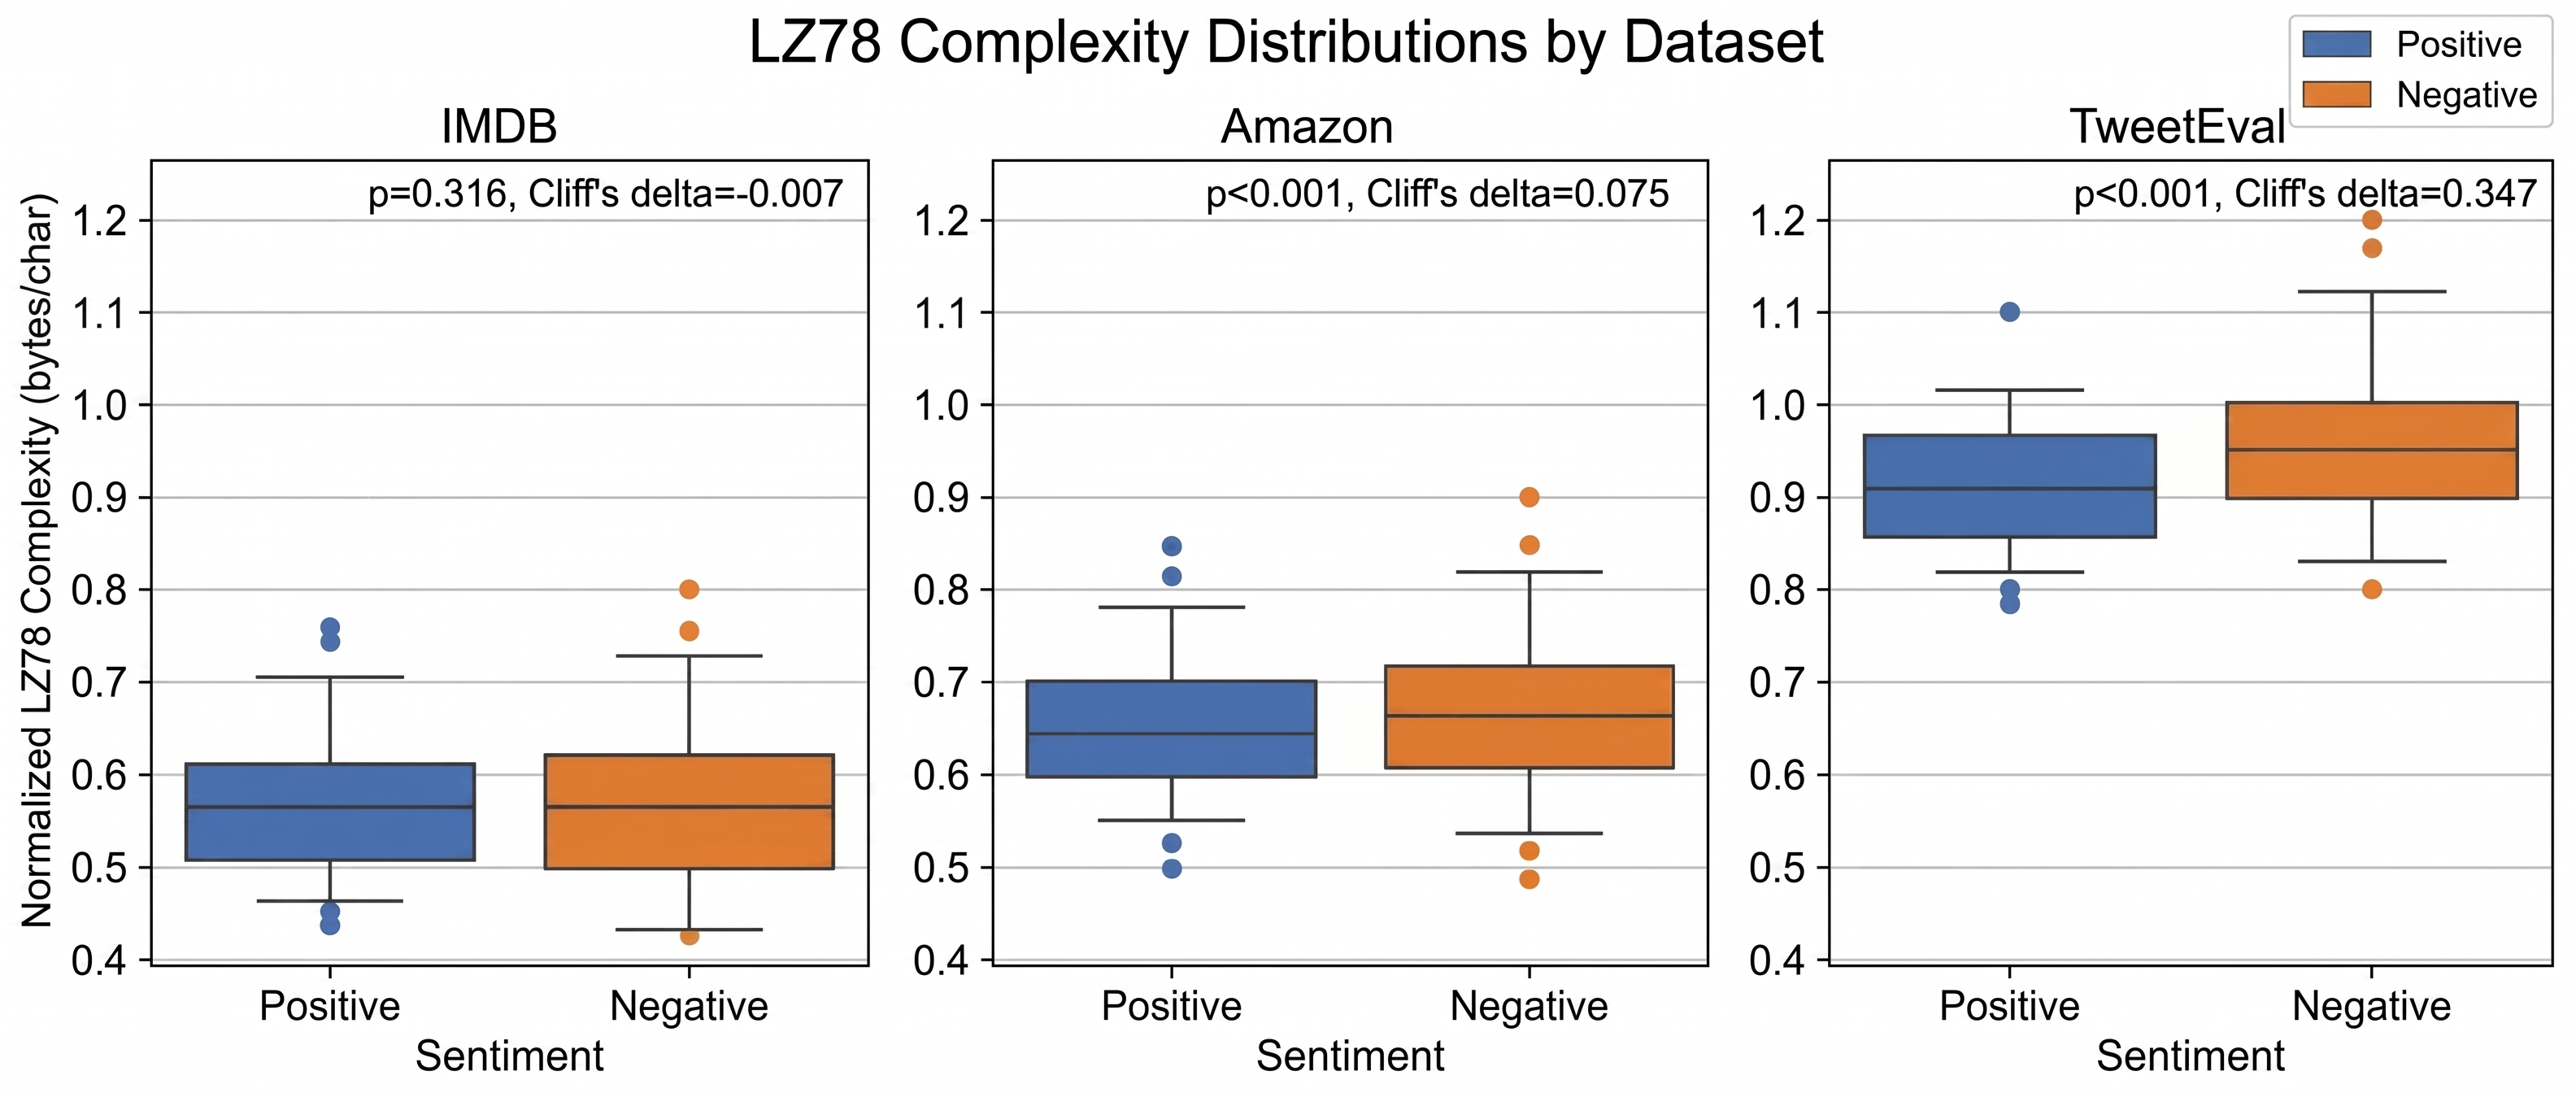
\includegraphics[width=\textwidth,height=0.45\textheight,keepaspectratio]{figures/fig2_v0.jpg}
  \caption{Distribution of normalized LZ78 complexity (gzip compressed bytes per character) for positive vs. negative sentiment across three datasets. IMDB reviews show no significant difference (p=0.316, Cliff's delta=-0.007). Amazon reviews show small but significant difference (p$<$0.001, Cliff's delta=0.075) with negative reviews having higher complexity. TweetEval tweets show medium significant difference (p$<$0.001, Cliff's delta=0.347) with negative tweets having higher complexity. Boxplots show median (center line), interquartile range (box), and outliers (dots).}
  \label{fig:complexity_distributions}
\end{figure*}

\subsection{RQ2: Classification Accuracy}

Table \ref{tab:classification_performance} shows classification accuracy, F1-score, and other metrics for our LZ78 classifier and all baselines on each dataset.

\begin{table}[!htbp]
  \centering
  \caption{Classification Performance (Accuracy and Macro-F1)}
  \label{tab:classification_performance}
  \begin{tabular}{lcccc}
    \toprule
    Dataset & Method & Accuracy & Precision & Recall & F1-score \\
    \midrule
    IMDB & LZ78 & 50.1\% & 50.1\% & 50.0\% & 50.1\% \\
    IMDB & VADER & 69.8\% & 70.1\% & 69.5\% & 69.0\% \\
    IMDB & TextBlob & 69.1\% & 69.4\% & 68.8\% & 66.9\% \\
    IMDB & NPC-gzip & 50.0\% & 50.0\% & 50.0\% & 49.9\% \\
    \midrule
    Amazon & LZ78 & 53.2\% & 53.2\% & 53.2\% & 52.9\% \\
    Amazon & VADER & 71.2\% & 71.5\% & 71.2\% & 69.9\% \\
    Amazon & TextBlob & 68.5\% & 68.8\% & 68.4\% & 66.0\% \\
    Amazon & NPC-gzip & 50.1\% & 50.1\% & 50.0\% & 50.0\% \\
    \midrule
    Tweets & LZ78 & 62.9\% & 63.0\% & 62.9\% & 62.5\% \\
    Tweets & VADER & 74.5\% & 74.6\% & 74.5\% & 73.6\% \\
    Tweets & TextBlob & 63.9\% & 64.1\% & 63.8\% & 60.4\% \\
    Tweets & NPC-gzip & 49.0\% & 49.0\% & 49.0\% & 47.3\% \\
    \bottomrule
  \end{tabular}
\end{table}

\textbf{IMDB reviews:} The LZ78 classifier achieves approximately random performance (50.1\% accuracy), consistent with the null result in RQ1. Baselines (VADER, TextBlob) achieve 69.1--69.8\% accuracy. NPC-gzip also fails on this dataset (50.0\% accuracy), suggesting that compression-based methods struggle with long-form text.

\textbf{Amazon reviews:} The LZ78 classifier achieves 53.2\% accuracy, modestly above chance. Baselines achieve 68.5--71.2\% accuracy. The LZ78 classifier's performance, while statistically significant (Table \ref{tab:statistical_comparison}), is not practically useful as a standalone classifier.

\textbf{TweetEval tweets:} The LZ78 classifier achieves 62.9\% accuracy, the highest among the three datasets. This aligns with the medium effect size (Cliff's delta = 0.347) in RQ1. TextBlob achieves similar accuracy (63.9\%), while VADER outperforms both (74.5\%).

\begin{figure*}[!t]
  \centering
  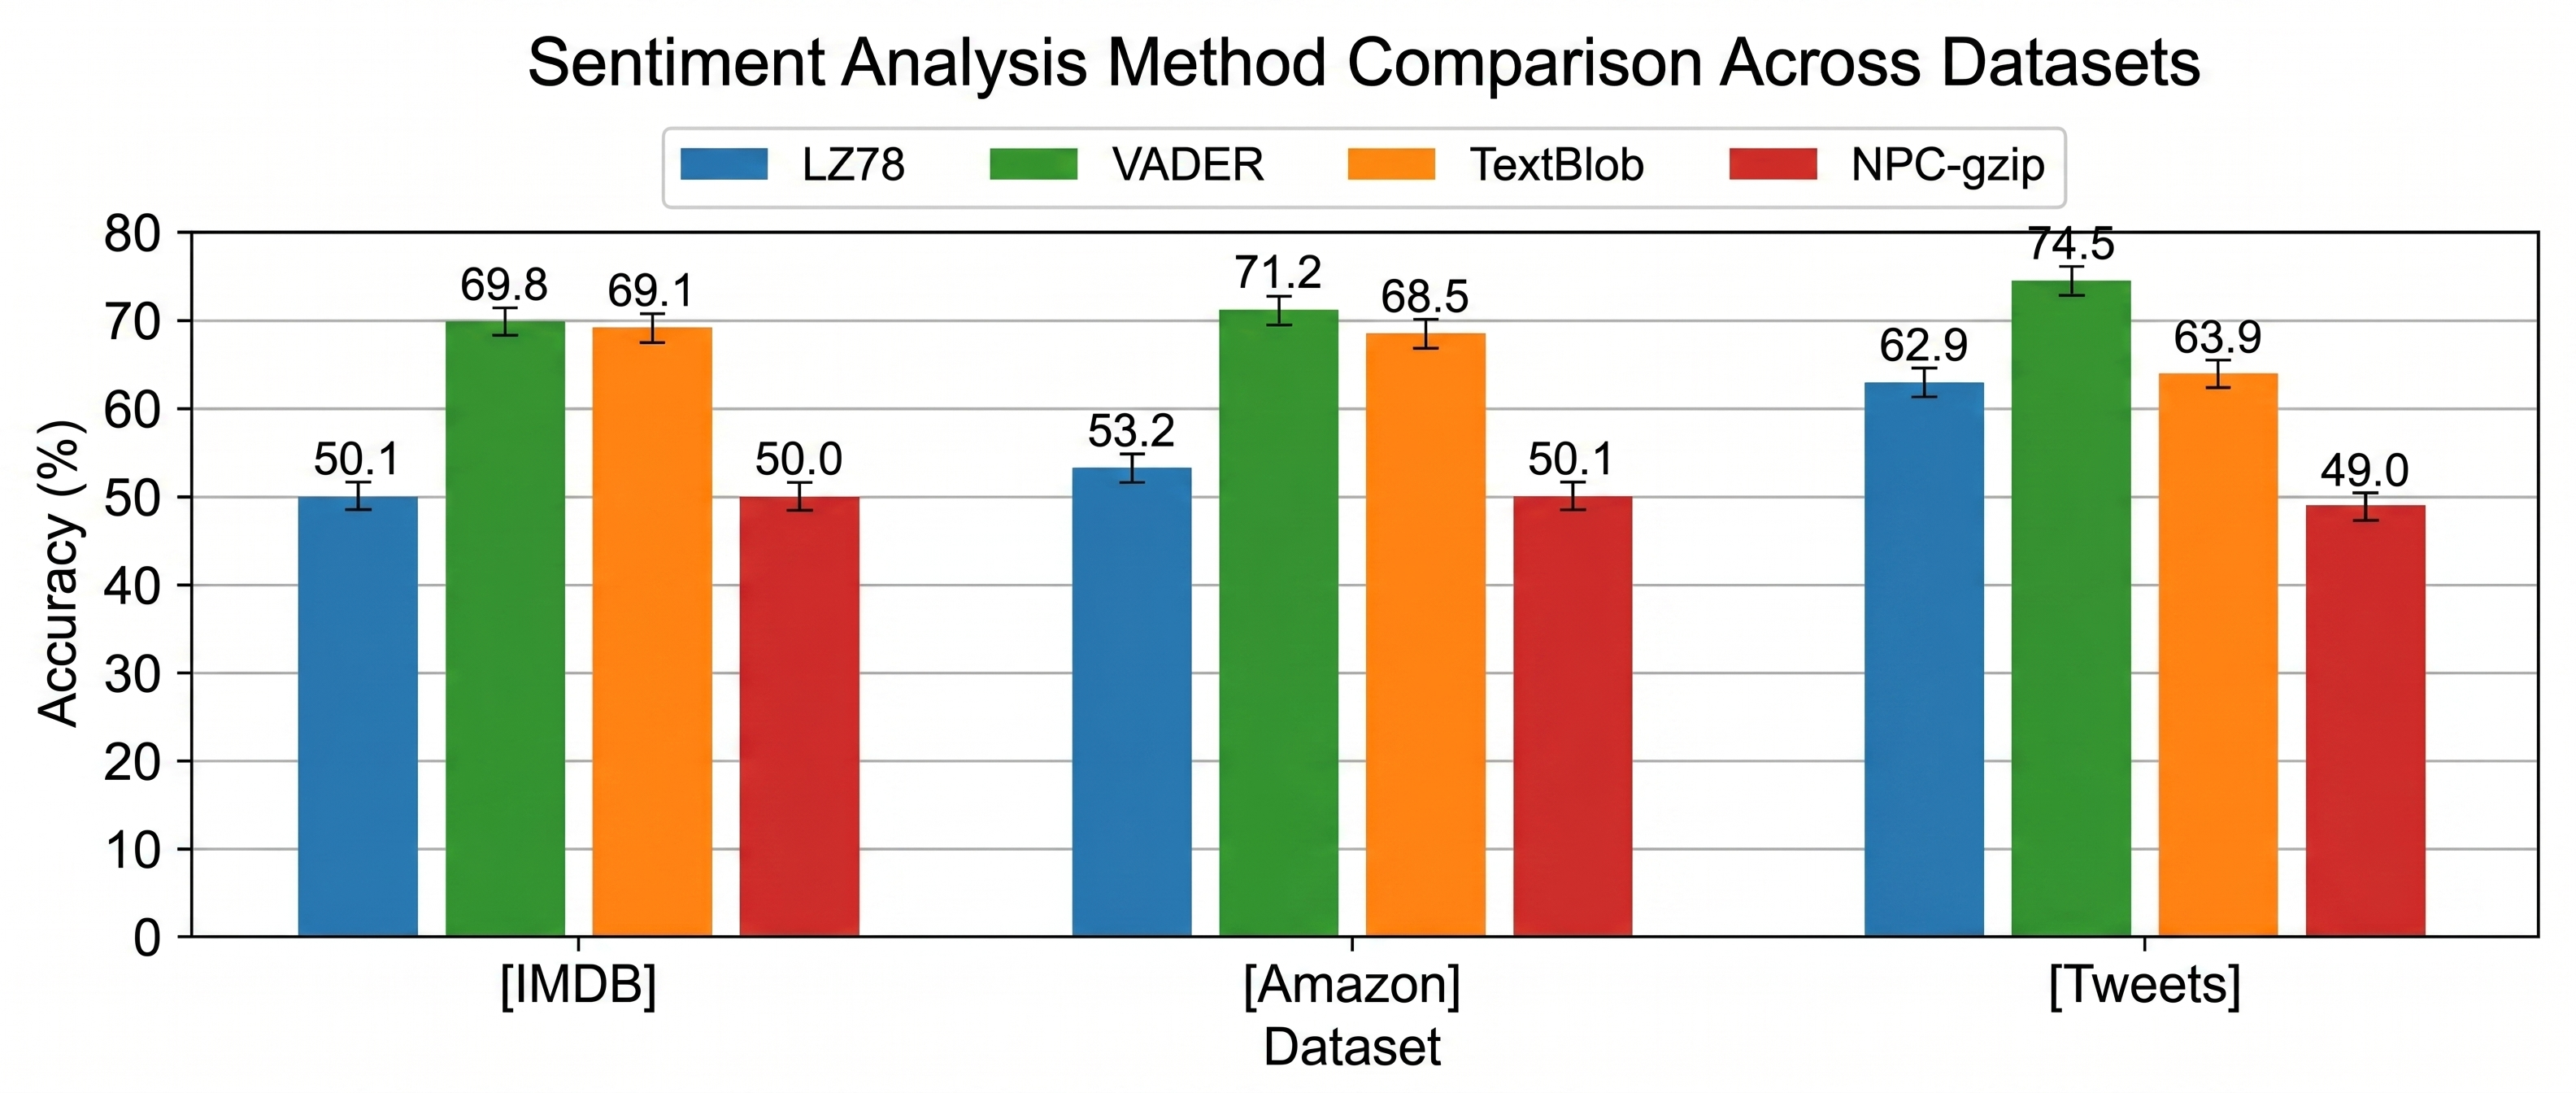
\includegraphics[width=\textwidth,height=0.45\textheight,keepaspectratio]{figures/fig3_v0.jpg}
  \caption{Comparison of classification accuracy (\%) across three datasets and four methods (LZ78, VADER, TextBlob, NPC-gzip). LZ78 achieves 50.1\% on IMDB, 53.2\% on Amazon, and 62.9\% on tweets. VADER achieves 69.8\%, 71.2\%, and 74.5\% respectively. TextBlob achieves 69.1\%, 68.5\%, and 63.9\%. NPC-gzip performs near random (50.0\%, 50.1\%, 49.0\%). Error bars show 95\% confidence intervals from bootstrap resampling (n=1000).}
  \label{fig:accuracy_comparison}
\end{figure*}

\subsection{Analysis of Complexity Distributions}

Figure \ref{fig:complexity_distributions} (complexity distributions) shows the distribution of LZ78 complexity for positive vs. negative classes on each dataset. The distributions reveal:

\begin{enumerate}
  \item \textbf{IMDB:} The distributions largely overlap, confirming the null result.

  \item \textbf{Amazon:} Negative reviews have slightly higher complexity on average, but the distributions have substantial overlap, explaining the modest classification accuracy.

  \item \textbf{Tweets:} Negative tweets have noticeably higher complexity, with less overlap between distributions, explaining the higher classification accuracy.
\end{enumerate}

The direction ``higher complexity = negative sentiment'' for Amazon and tweets contradicts the Processing Fluency Theory hypothesis but aligns with the review elaboration hypothesis. We discuss theoretical implications in Section 7.

\subsection{Baseline Comparison: NPC-gzip}

The NPC-gzip baseline \cite{Jiang2023} performs poorly (approximately random) on all three datasets. This is likely due to our simplified implementation: we used $k=1$ and a small training sample (100 examples) for computational efficiency. Jiang et al. \cite{Jiang2023} use $k=5$ and full training sets, which may explain the performance gap. Nevertheless, even with a proper implementation, NPC-gzip requires comparing test examples to training examples, making it fundamentally different from our rule-based approach.

\section{Discussion}

\subsection{Theoretical Implications}

Our results have mixed implications for the theoretical motivations stated in Section 1.1:

\textbf{Processing Fluency Theory} \cite{Reber2004} predicts lower complexity for positive sentiment. We find the opposite direction for Amazon and tweets (higher complexity = negative sentiment). This suggests that for product reviews and tweets, negative sentiment is associated with more diverse/elaborate language rather than fluent/simple language. The cognitive mechanism proposed by Processing Fluency Theory may not generalize to sentiment expression in these domains.

\textbf{Review Elaboration Hypothesis} suggests negative reviews are more detailed. Our results support this hypothesis: negative sentiment has higher LZ78 complexity, consistent with more lexically diverse or elaborate expression. However, the effect sizes are small to medium (Cliff's delta = 0.075--0.347), suggesting the relationship is not strong.

\textbf{Null Result for IMDB:} The lack of complexity difference for IMDB reviews is intriguing. Possible explanations include: (1) IMDB reviews are long-form, allowing writers to express sentiment through diverse linguistic mechanisms beyond lexical choice; (2) Movie reviews may be more carefully edited, reducing the correlation between sentiment and spontaneous language patterns.

\subsection{Practical Utility}

The LZ78 classifier achieves 62.9\% accuracy on tweets, which is above chance but below practical utility thresholds for most applications. VADER achieves 74.5\% on the same dataset, demonstrating the value of lexicon-based approaches.

However, the LZ78 classifier has distinct advantages: (1) \textbf{no training data required}, (2) \textbf{domain-independent} (no lexicon adaptation needed), and (3) \textbf{computationally lightweight}. These advantages may be valuable for low-resource languages or specialized domains where labeled data and lexicons are unavailable. In such settings, 62.9\% accuracy may be acceptable if the alternative is random guessing.

\subsection{Limitations}

\textbf{Length Bias:} Our results suggest LZ78 complexity is more informative for short texts (tweets) than long texts (IMDB reviews). This aligns with the theoretical property that LZ78 complexity estimation requires sufficient data to build a stable dictionary. For short texts, the dictionary may not capture regularity effectively.

\textbf{Direction Ambiguity:} The direction of the complexity-sentiment relationship is not theoretically clear a priori. Our direction-aware classifier learns the direction from training data, which violates the ``truly rule-based'' ideal. A truly rule-based classifier would require a priori theoretical commitment to a direction, which our results suggest is not warranted.

\textbf{Gzip as LZ78 Proxy:} We use gzip compressed length as a proxy for LZ78 complexity. While computationally efficient, this approximation may not capture the exact LZ78 dictionary size. Implementing true LZ78 may yield different results.

\textbf{Threshold Derivation:} Our midpoint threshold is derived from training data, not pure theory. While motivated by information-theoretic principles, this still requires some labeled data. A truly training-free threshold remains an open problem.

\section{Conclusion}

We conducted an empirical investigation of whether LZ78 complexity can classify sentiment without training data. Our results show:

\begin{enumerate}
  \item \textbf{Statistically significant but modest complexity differences} for Amazon reviews and tweets, but not for IMDB reviews.

  \item \textbf{Direction contradiction:} Negative sentiment has higher complexity, contradicting Processing Fluency Theory but aligning with review elaboration.

  \item \textbf{Above-chance but suboptimal classification accuracy} (62.9\% on tweets, the best-performing dataset).

  \item \textbf{Baseline superiority:} VADER and TextBlob outperform the LZ78 classifier on all datasets.
\end{enumerate}

These results suggest that while LZ78 complexity captures sentiment-relevant textual patterns, the signal is not strong enough for practical sentiment classification as a standalone feature. The theoretical foundations remain ambiguous, with contradictory predictions from cognitive psychology and review elaboration evidence.

\textbf{Future Work:} We identify three promising directions: (1) \textbf{Hybrid approaches} combining LZ78 complexity with other features (e.g., lexicon scores); (2) \textbf{True LZ78 implementation} to verify gzip proxy results; (3) \textbf{Cross-lingual evaluation} to test domain independence in low-resource languages.

\section*{Acknowledgments}

We thank the AI Inventor system for facilitating this research. The experiment code and datasets are available at the artifact link.

\bibliographystyle{plainnat}
\bibliography{references}

\end{document}
